\chapter{Analysis}
\label{chap:analysis}

We now describe the analyses we performed on the data in this chapter. The chapter begins by discussing the ways we arrived at the calculations made on the data, the details of how these tasks were performed using the data described in \chapref{chap:data} and then goes on the discuss the results and the consequent conclusions derived from the results.

Our goal is to investigate what proportion of the indicative tweets that we extracted can be found in the articles that they link to, in order to determine whether indicative tweet generation can be viewed as an extractive summarization problem. \tabref{tab:noextract} gives an example of data where the tweet that was shared about the article does not come directly from the article text, while \tabref{tab:extract} shows a tweet that was almost entirely extracted from the text of the article, but changed a little for the purpose of readability.

\begin{table}[!htbp]
\centering
\begin{tabular}{|p{0.1\linewidth}|p{0.8\linewidth}|}
\hline
Tweet &  Are \#Airlines doing enough with \#Ebola? http://t.co/XExWwxmjnk \#travel \\ \hline
Title &  Could shortsighted airline refund policies lead to an outbreak? \\  \hline
Text  &  The deadly Ebola virus has arrived in the United States just in time for the holiday travel season, carrying fear and uncertainty with it... \\ \hline
\end{tabular}
\captionof{table}{Example of a tweet, title of the article and the text when tweet cannot be extracted from text.}
\label{tab:noextract}
\end{table}

\begin{table}[!htbp]
\centering
\begin{tabular}{|p{0.1\linewidth}|p{0.8\linewidth}|}
\hline
Tweet & Officer \textbf{Wilson will be returned to active duty if no indictment}, says \#Ferguson Police \textbf{Chief} http://t.co/zrRIBxMUYJ  \\ \hline
Title & Jackson clarifies comments on Wilson's future status \\ \hline
Text  & ...\textbf{Chief} Jackson said if the grand jury does \textbf{not indict Wilson}, he \textbf{will} immediately \textbf{return to active duty}.... \\ \hline
\end{tabular}
\captionof{table}{Example of a tweet, title of the article and the text when tweet can be extracted from text. The matched portions of the tweet and article are in bold.}
\label{tab:extract}
\end{table}

We first compute the proportion of tweets that can be recovered directly from the article in its entirety (\secref{sec:exact-match}). Then, we calculate the degree of overlap in terms of unigrams and bigrams between the tweet and the text of the document (Sections \ref{sec:unigrams}, \ref{sec:bigrams}). 

In addition, we consider locality within the article when computing the overlap. For the unigram analysis, we performed a variant of the analysis, in which we computed the overlap within three-sentence windows in the source article (\secref{sec:window}). We also compute the least common subsequences between the tweet and the document (\secref{sec:lcs}). This was done to investigate whether sentence compression techniques could be applied to local context windows to generate the tweet.

These calculations are analogous to the ROUGE-1, -2 and -L style calculations. These results give an indication of the degree to which the tweet is extracted from the document text. 

For all these analyses, the stop words have been eliminated from the tweet as well as the document, so that only the informative words are taken into consideration. The comparisons were made without lemmatization or stemming, to adhere closely to existing work in extractive summarization, where the only modifications to the source text are removing discourse cue words or removing words by sentence compression techniques. The hashtags, references (@) and URLs from the tweets were all removed for analysis.

\section {Exact Match Calculations}
\label{sec:exact-match}
We first checked for a complete substring match of the tweet in the text. Out of the 2471 unique instances of tweet and article pairs, a complete match was found only 23 times. In 9 cases out of these, the tweet text matched the title of the article, which our preprocessing tool did not correctly separate from the body of the article. In the other cases, the text of the tweet appears in its entirety inside the body of the article. This suggests that the user chose the sentence that either seemed to be the most conclusive contribution of the article, or expressed the opinion of the user to be tweeted. An example for this is detailed in \tabref{tab:fullextract}.

Apart from the 9 times where the tweet was matched with title in the article, we also checked to see if the tweet text matched with the article titles that were separately extracted by the \texttt{newspaper} package in order to determine if tweets could be generated using the headline generation methods. We found that it did not match with the titles. However, even though there are no exact matches, there might still be matches where the tweet is a slight modification of the headline of the article, and can be measured using a partial match measure.

\begin{table}[!htbp]
\centering
\begin{tabular}{|p{0.1\linewidth}|p{0.8\linewidth}|}
\hline
Tweet &  @PNHP: \textbf{6. Renounce punitive and counterproductive measures such as “sealing the borders,”} http://t.co/LRLS2MhPRE \#Ebola \\ \hline
Title & Physicians for a National Health Program \\  \hline
Text  & As health professionals and trainees, we call on President Obama to take the following immediate steps to address the Ebola crisis... \textbf{6. Renounce punitive and counterproductive measures such as “sealing the borders,”} and take steps to address the... \\ \hline
\end{tabular}
\captionof{table}{Example where tweet is extracted as is from the text, matched portion in bold.}
\label{tab:fullextract}
\end{table}


\begin{figure}[!htbp]
\centering
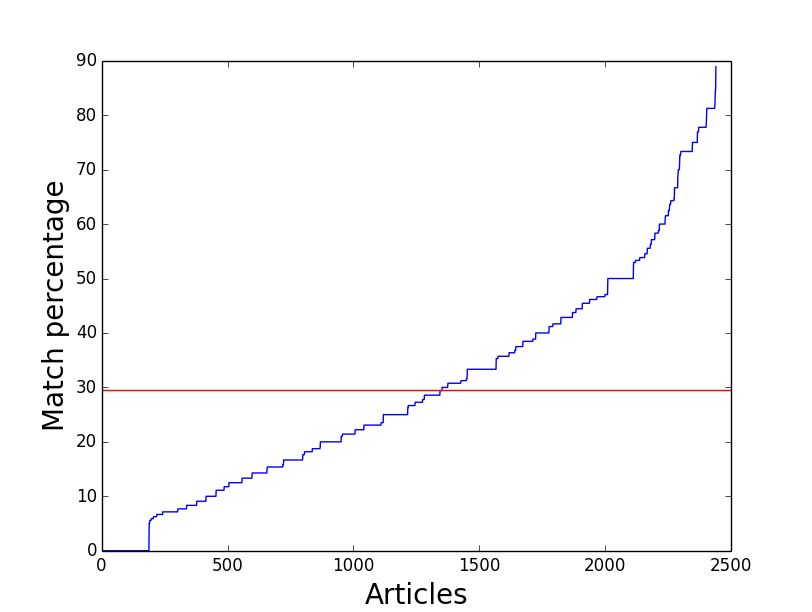
\includegraphics[width=0.7\textwidth, height=9cm]{unigrammatch}
\caption[Unigram matching percentages]{Distribution of unigram match percentage over unique tweets and articles. The mean is 29.53\%, indicated by the red horizontal line, with a standard deviation of 20.2\%}
\label{fig:unigrammatch}
\end{figure}


\begin{figure}[!htbp]
\centering
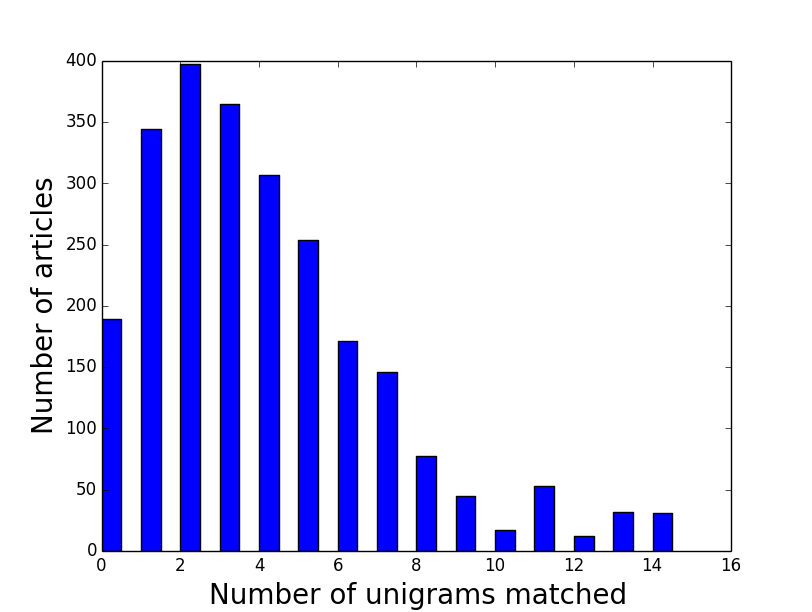
\includegraphics[width=0.7\textwidth, height=9cm]{num_unigrams}
\caption[Histogram for number of unigrams matched]{Histogram of number of unique tweet-article pairs vs number of unigrams matched. The mean number of unigrams matched per tweet-article pair is 3.9.}
\label{fig:num_unigrams}
\end{figure}


\section{Percentage Match for Unigrams}
\label{sec:unigrams}

Next, we computed the percentage match between the text of the tweet and the text in the article. This was a bag-of-words check using unigram overlap between the tweet and the document. Let $\textit{unigrams}(x)$ be the set of unigrams for some text $x$, then $u$, the percentage of matching unigrams found between a given tweet, $t$ and a given article, $a$, can be defined as  

\begin{equation}
u = \frac{| \textit{unigrams}(t) \cap \textit{unigrams}(a) |}{| \textit{unigrams}(t) |} * 100
\end{equation}

\figref{fig:unigrammatch} shows the percentage of matches in the tweet and the article text as compared to the number of unigrams in the tweet. The mean match percentage is 29.53\% and standard deviation is 20.2\%. The mean of this distribution shows that the number of matched unigrams from a tweet in the article are fairly low. \figref{fig:num_unigrams} shows the number of articles with a certain number of matching unigrams. The graph shows that the most common number of unigrams matched was 2. The number of articles continues to decrease with higher unigrams matched. The slight rise at the end - more than 10 matched unigrams - is accounted for by the completely matched tweets described above.

\begin{figure}[!htbp]
\centering
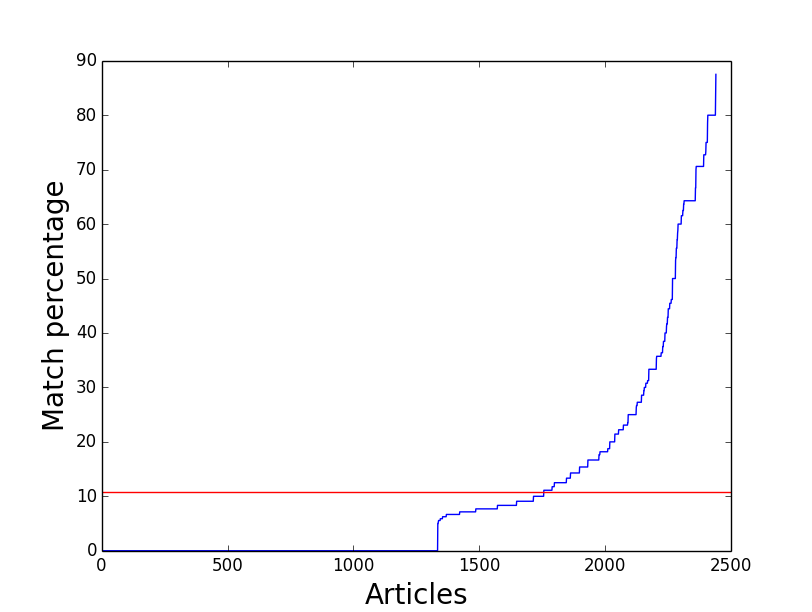
\includegraphics[width=0.7\textwidth, height=9cm]{bigrammatch}
\caption[Bigram match percentages]{Distribution of bigram match percentage over the tweet-article pair. The mean here is 10.73\% shown by the red horizontal line, with a standard deviation of 18.5\%}
\label{fig:bigrammatch}
\end{figure}


\section{Percentage Match for Bigrams}
\label{sec:bigrams}

Similar to the unigram matching techniques, the bigram percentage matching was also calculated. The text of the tweet was converted into bigrams and we then looked for those bigrams in the article text. The percentage was calculated similar to the unigram matching done earlier. For the set of bigrams for a text $x$, $\textit{bigrams}(x)$, percentage of matching bigrams $b$ for the tweet $t$ and article $a$ is: 

\begin{equation}
b = \frac{| \textit{bigrams}(t) \cap \textit{bigrams}(a) |}{| \textit{bigrams}(t) |} * 100
\end{equation}

\figref{fig:bigrammatch} shows the percentages of matched bigrams found. The mean is 10.73 with a standard deviation of 18.5. As seen in the figure, most of the tweet-article pairs have no matched bigrams. The percentage then increases to reflect the complete matches found above.

\begin{figure}[!htbp]
\centering
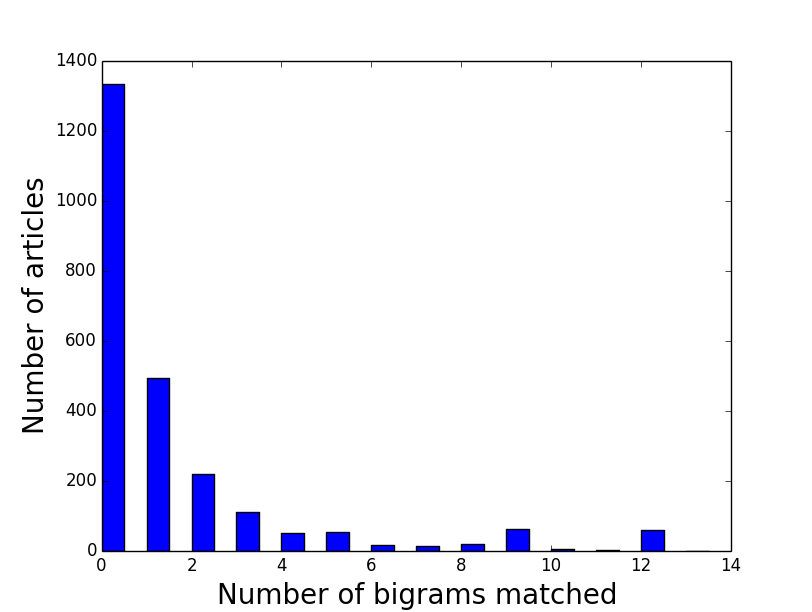
\includegraphics[width=0.7\textwidth, height=9cm]{num_bigrams}
\caption[Histogram for number of matched bigrams.]{Histogram of number of unique tweet-article pairs vs number of bigrams matched. The mean number of bigrams matched per article is 1.9.}
\label{fig:num_bigrams}
\end{figure}

\figref{fig:num_bigrams} shows frequency of the number of tweet-article pairs for the number of bigrams matched. There are no matched bigrams for most of the pairs. A smaller number of articles had one matched bigram, and the number decreased until the end, where it increases a little at more than 10 matched bigrams because of exact tweet matches. 


\section{Percentage Match Inside a Window in the Article Text}
\label{sec:window}

The next analysis checks for a significant word matching inside a three-sentence window inside the article text. We used a three sentence long window using the sentence boundary information obtained during preprocessing. A window of three sentences was chosen to give a smaller context for the tweet to be extracted from than the entire article. The number was chosen as a moderate context window size as not too small to reduce it to a sentence level, and not too big for the context to be diluted. This was done to investigate whether a pseudo-extractive multi-sentence compression approach could convert a small number of sentences into a tweet.

After the text of the window was extracted, we performed a similar analysis as the last one, except on a smaller set of sentences. The matching percentages from all three-sentence windows in the articles were computed and the maximum out of these was taken for the final results. Let a sentence window $w_i$ be the set of three consecutive sentences starting from the sentence number $i$. For this window, the unigram match in the tweet $t$, and the window is the unigram match $u$ calculated above. Then, the maximum match from all the windows, $uw$ is 

\begin{equation}
uw = max_{w_i \in S} u(t, w_i)
\end{equation}

\begin{figure}[!htbp]
\centering
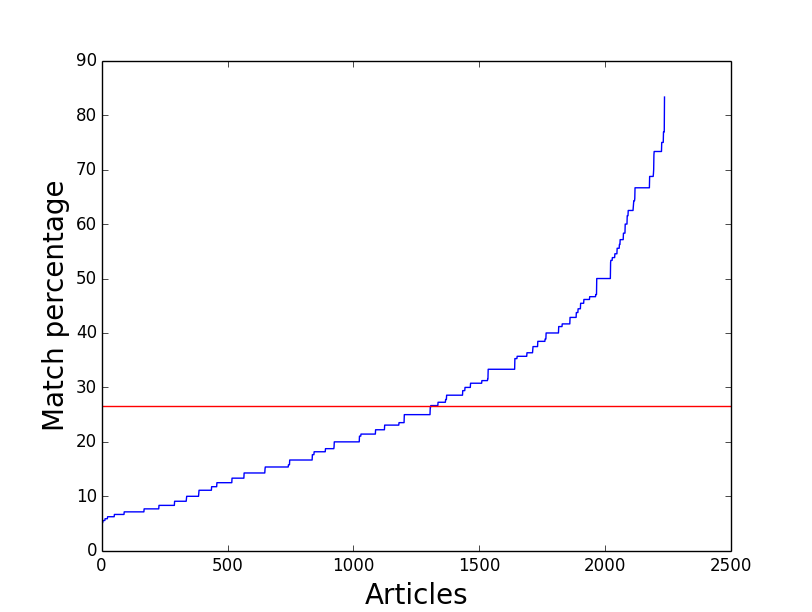
\includegraphics[width=0.7\textwidth, height=9cm]{unigramwindow}
\caption[Match percentages in tweet against window in article]{Percentages of common words in tweet and a three sentence window in the article. The maximum match from all percentages is chosen for an article. The red horizontal line is the mean is 26.6\%, and standard deviation 17\%.}
\label{fig:unigramwindow}
\end{figure}

The result from this experiment is shown in \figref{fig:unigramwindow}. Here, the mean of the values is 26.6\% and deviation 17\%. Again this shows that only a small proportion of tweets can be generated even with an approach that combines unigrams from multiple sentences in the article.


\section{Longest Common Subsequence Match Inside a Window for the Text}
\label{sec:lcs}

\begin{figure}[!htbp]
\centering
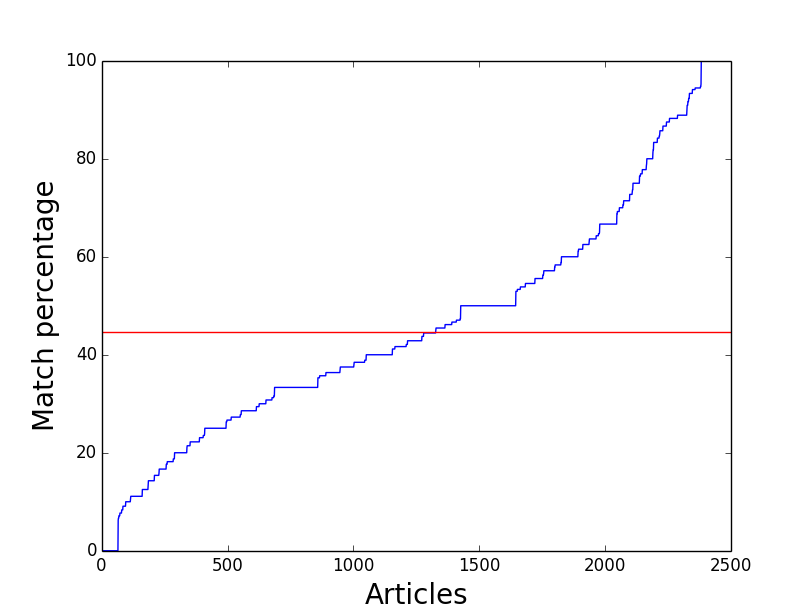
\includegraphics[width=0.7\textwidth, height=9cm]{lcs_doc}
\caption[LCS match percentages]{Percentages of words matching in tweet and document text using an LCS algorithm. Mean is 44.6\%, which is shown by the red horizontal line, and standard deviation is 22.7\%.}
\label{fig:lcs}
\end{figure}

The percentage match analyses were a bag-of-words approach that disregarded the order of the words inside the texts and tweets. To respect the order of the words in the sentence of the tweet, we also used the least common subsequence algorithm between the tweet text and the document text. This subsequence matching was done inside a sentence window of 5 sentences. 
Again, the final result for the article was the window in which the maximum percentage was recorded among all windows. The percentage match was calculated using the number of words in the tweet as the denominator.

If $\textit{lcs(t, a)}$ is the longest common subsequence between the tweet $t$ and article $a$, $\textit{unigrams}(x)$ is the set of unigrams for a text $x$, then the percentage of match for the lcs as compared to the tweet, $\textit{l}$ is


\begin{equation}
l = \frac{| \textit{lcs}(t, a) |}{| \textit{unigrams}(t) |} * 100
\end{equation}


 These numbers are shown in \figref{fig:lcs}. The mean here is 44.6\% and the standard deviation is 22.7\%. 

\section{Interaction with Formality}

As seen in the results of the analyses performed above, the tweets have little in common with the articles they are linked to. This shows that extractive summarization algorithms can only recover a small proportion of the indicative tweets. To tie in the results of the findings above with some intuitive notions about the text and see how formality interacts with the results, we also calculated the formality of the articles. This formality score was correlated with the longest common subsequence measure that we defined above. 

We assume that the formality of an article can be estimated by the formality of the words and phrases in the article. We used the formality lexicon of \cite{brooke2013multi}. They calculate formality scores for words and sentences by training a model on a large corpus based on the appearance of words in specific documents. Their model represents words as vectors and the formal and informal seeds appear in opposite halves of the graphs, suggesting that we can use these seeds to determine if an article is formal or informal. The lexicon consists of words and phrases and their degree of formality. Thus, more formal words are marked on a positive scale and informal words like those occurring in colloquial language are marked on a negative scale. 

Let the set of formality expressions from the lexicon be $L$, and the formality score for an expression $e$ be $\textit{score}(e)$. Let the set of all substrings from the article $\textit{substrings}(a)$ be $S$. Then, the formality score $f$ for an article $a$ is the number of formal expressions per 10 words in article is   

\begin{equation}
f = \frac{\sum\limits_{e \in L \& e \in S} \textit{score}(e)}{| \textit{unigrams}(a) |} * 10
\end{equation}

The formality lexicon gave positive weights for formal expressions and negative for informal expressions. When we computed $f$ using both formal and informal expressions, we found that the informal words predominated and ``swamped'' the signal of the formal words, leading to incomprehensible results. Thus, we discarded the informal words and used only the weights from the formal words in our final calculations. To check that these formality scores made sense intuitively, we calculated the average formality score for the articles belonging to each hashtag and ordered them, as shown in \tabref{tab:formal}.

\begin{table}[!htbp]
\centering
\begin{tabular}{|l|l|}
\hline
Lowest  & Highest  \\ \hline
\#theforceawakens       & \#KevinVickers           \\
\#TaylorSwift           & \#erdogan                \\
\#winteriscoming        & \#apec                  \\ \hline
\end{tabular}
\caption[Order of formality ranking in hashtags]{Table of hashtags (broadly, topics) with highest and lowest formality according to the lexicon.}
\label{tab:formal}
\end{table}


\begin{table}[!htbp]
\centering
\begin{tabular}{|p{0.1\linewidth}|p{0.8\linewidth}|}
\hline
Tweet &  @globetoronto: Why Buffalo got clobbered with snow and Toronto did not. \#weather \#snowstorm http://t.co/gcwwoDPZmX... http://t.co/BXY7EH6F3u" \\ \hline
Title & What caused Buffalo’s massive snow and why Toronto got lucky \\  \hline
Text  & Torontonians have long been the butt of jokes about calling in the army every time a few snow flurries whip by... \\ \hline
\end{tabular}
\caption[Example of formality in article affecting tweet]{Example of a tweet, title of the article where the formality of the article is over the mean, and the tweet is extracted from the article.}
\label{tab:formalexample}
\end{table}

This formality score for each article was correlated with the percentage of match obtained using the longest common subsequence algorithm. The Pearson correlation value was 0.41, with a p-value of 7.08e-66, indicating that the interaction between formality and overlap was highly significant. Hence, we can say that the more formal the subject or the article, the better the tweet can be extracted from the article. \tabref{tab:formalexample} gives an example of the formality of the article, which is a low 4.2 formality words per 10 words, where the tweet is not extracted from the article, but rephrased from the article instead.

We speculate that tweets associated with less formal articles may contain more abbreviations and non-standard words or spellings, which decreases the amount of overlap. To counter this case, we tried experimenting with word normalization systems which could resolve words like `2mw' or `4eva' to `tomorrow' and `forever' respectively. Systems described by \cite{yang2013log} and \cite{gouws2011contextual} were tested with our data. Unfortunately, neither provided the results that were suitable enough to integrate with our analyses, and this remains something to look into further upon development of more accurate word normalization systems. 

